\subsection{Kiến thức về Local Binary Patterns (LBP)}

\subsubsection*{Đặc trưng ảnh cục bộ (Local Image Texture)}
Dấu của hiệu giá trị các pixel xung quanh so với điểm ảnh ở tâm sẽ bất biến với phép chiếu sáng.

\begin{equation}
	T \sim t(s(g_0-g_c), s(g_1-g_c),\ldots,s(g_{P-1} - g_c))
\end{equation}

Có 2 kiểu đặc trưng cục bộ:
\begin{itemize}
	\item \textit{Vuông (Square Neighborhood):} Các điểm trên vùng đặc trưng cục bộ xếp thành hình vuông (đi theo chiều vòng tròn lượng giác), điểm $g_0$ cách điểm $g_c$ một khoảng R (bán kính) pixel. 
	\item \textit{Tròn (Circular Neighborhood):} Các điểm trên vùng đặc trưng cục bộ xếp thành hình tròn (đi theo chiều vòng tròn lượng giác), điểm $g_0$ cách điểm $g_c$ một khoảng R (bán kính) pixel. Do xếp theo hình tròn nên sẽ có một số điểm phải sử dụng phép nội suy để tính. Trong các nội dung bên dưới, xin sử dụng đặc trưng tròn để bàn.
\end{itemize}
\begin{figure}[H]
	\begin{center}
		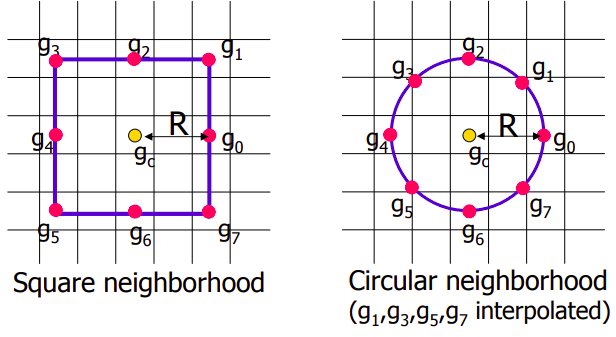
\includegraphics[scale=0.6]{images/theo1/local_image_texture}
		\caption{Đặc trưng vuông bên trái, đặc trưng tròn bên phải}
	\end{center}
\end{figure}
\pagebreak

\subsubsection{LBP\textsubscript{P,R} (1996)}

$LBP_{P,R}$ xác định giá trị tại điểm ảnh $g_c$ bằng đặc trưng ảnh cục bộ của các điểm xung quanh điểm ảnh đó qua công thức:
\begin{equation}
	LBP_{P,R} = \sum^{P-1}_{p=0}{s(g_p-g_c)\times 2^p}
\end{equation}
Trong đó:
\begin{itemize}
	\item \textit{P(Point)} là số lượng điểm trong vùng đặc trưng cục bộ, mỗi điểm cách nhau một khoảng $\frac{2\pi}{P}$ rad.
	\item \textit{R(Radius)} là bán kính của vùng đặc trưng cục bộ.
	\item $g_c$ là điểm cần tính giá trị $LBP_{P,R}$ (Tâm của hình vuông hay hình tròn).
	\item $g_p$ là điểm thứ p trên vùng đặc trưng cục bộ.
	\item \textit{s (sign function)} là hàm dấu:
		\begin{equation}
			s(x) = \begin{cases}
				1, & x \geq 0\\
				0, & x < 0
			\end{cases}
		\end{equation}
\end{itemize}

\textit{Ví dụ}: Giá trị của $LBP_{8,1}$ của điểm ảnh ở giữa (hình 2) được tính như sau:
$$
	LBP_{8,1} = \sum^{7}_{p=0}{s(g_p-76)\times 2^p} = 1 + 2 +2^3 + 2^5 + 2^6 = 107
$$

\begin{figure}[H]
	\begin{center}
		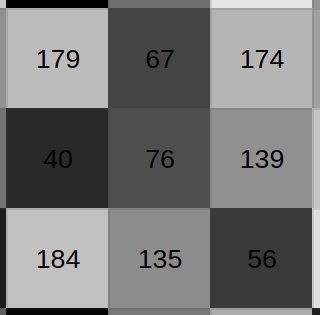
\includegraphics[scale=0.5]{images/theo1/LBP_exam1}
		\caption{Ví dụ $LBP_{P,R}$}
	\end{center}
\end{figure}
\pagebreak

\underline{Ưu điểm}
\begin{itemize}
	\item Bất biến với phép chiếu sáng. Giúp giảm FRR (False Reject Rate) cho các ảnh được chụp ở các điều kiện sáng tối khác nhau. \\
	\textit{Ví dụ}: Độ sáng tăng lên nhưng $LBP_{8,1}$ không thay đổi (Hình 3).
	$$
		LBP_{8,1} = \sum^{7}_{p=0}{s(g_p-76)\times 2^p} = 1 + 2 +2^3 + 2^5 + 2^6 = 107
	$$
	\begin{figure}[H]
		\begin{center}
			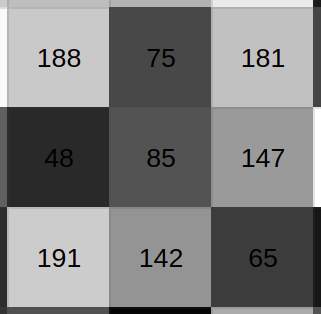
\includegraphics[scale=0.5]{images/theo1/LBP_exam2}
			\caption{$LPB_{P,R}$ bất biến phép chiếu sáng}
		\end{center}
	\end{figure}
	\item Không cần phải so sánh 2 vector đặc trưng (Công thức 1).
	\item Tính toán đơn giản.
\end{itemize}
\underline{Nhược điểm}
\begin{itemize}
	\item Không bất biến với phép xoay.\\
	\textit{Ví dụ:} khi xoay hình 90 độ theo ngược chiều kim đồng hồ, ta sẽ có giá trị $LBP_{8,1}$ thay đổi (Hình 3).
	$$
		LBP_{8,1} = \sum^{7}_{p=0}{s(g_p-76)\times 2^p} = 1 + 2^2 + 2^3 + 2^5 + 2^7 = 173
	$$
	\begin{figure}[H]
		\begin{center}
			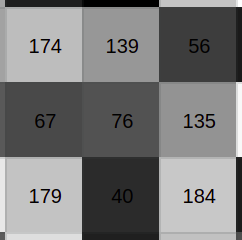
\includegraphics[scale=0.6]{images/theo1/LBP_exam3}
			\caption{$LBP_{P,R}$ không bất biến với phép xoay}
		\end{center}
	\end{figure}
\end{itemize}


\subsubsection{LBP\textsubscript{P,R}\textsuperscript{ri} (2000)}
Khắc phục được nhược điểm của $LBP_{P,R}$, $LBP_{P,R}^{\text{  }ri}$ bất biến với cả phép quay và phép chiếu sáng bằng cách sử dụng giá trị nhỏ nhất để đại diện cho tất cả các ảnh xoay (ảnh được xoay theo chiều đường tròn lượng giác với một góc không đổi).

\begin{equation}
	LBP_{8,1}^{\text{  }ri} = \min_{i=0 \to P-1}{ROR(LBP_{8,1}, i)}
\end{equation}
\textit{Trong đó:}
\begin{itemize}
	\item \textit{ROR(x, i)} là phép xoay bit sang phải của x theo vòng tròn i lần. Tương ứng với việc xoay tập hợp các hàng xóm theo chiều kim đồng hồ.
\end{itemize}

\textit{Ví dụ}: Giá trị của $LBP_{8,1}^{\text{  }ri}$ của điểm ảnh ở giữa (hình 2) được tính như sau:
\begin{align*}
	01101011_2 &= 107\\
	10110101_2 &= 181\\
	11011010_2 &= 218\\
	01101101_2 &= 109\\
	10110110_2 &= 182\\
	01011011_2 &= 91  \text{   (Nhỏ nhất)}\\
	10101101_2 &= 173\\
	11010110_2 &= 214\\
\end{align*}
$$
	\Longrightarrow LBP_{8,1}^{\text{  }ri} = \min_{i=0 \to P-1}{ROR(LBP_{8,1}, i)} = 91
$$
\subsubsection{LBP\textsubscript{P,R}\textsuperscript{riu2} (2002)}

Đặc trưng của $LBP_{P,R}^{\text{  }riu2}$ khắc phục được nhược điểm của $LBP_{P,R}^{\text{  }ri}$ đó là:
\begin{itemize}
	\item Tính toán nhanh và đơn giản. Với mỗi điểm ảnh, chỉ cần tính một giá trị.
	\item Sử dụng các \textit{Uniform Patterns} để  giảm các trường hợp phép xoay không mang lại nhiều ý nghĩa, do mỗi lần xoay cho các giá trị khác nhau làm không thể hiện đươc đặc thù của điểm ảnh.
\end{itemize}
\pagebreak

\textbf{Uniform Patterns:} Một mẫu nhị phân được gọi là đồng dạng khi xét chuỗi bit xoay vòng thì có nhiều nhất là 2 lần thay đổi (transitions) từ giá trị bit 0 sang 1 hoặc từ giá trị bit 1 sang 0. 

\textit{Ví dụ: }Với hàng đầu tiên là 9 mẫu \textit{Uniform}. Còn lại là các mẫu \textit{Non-Uniform}. Các mẫu Non-Uniform không mang lại nhiều ý nghĩa trong nhận dạng.
\begin{figure}[H]
	\begin{center}
		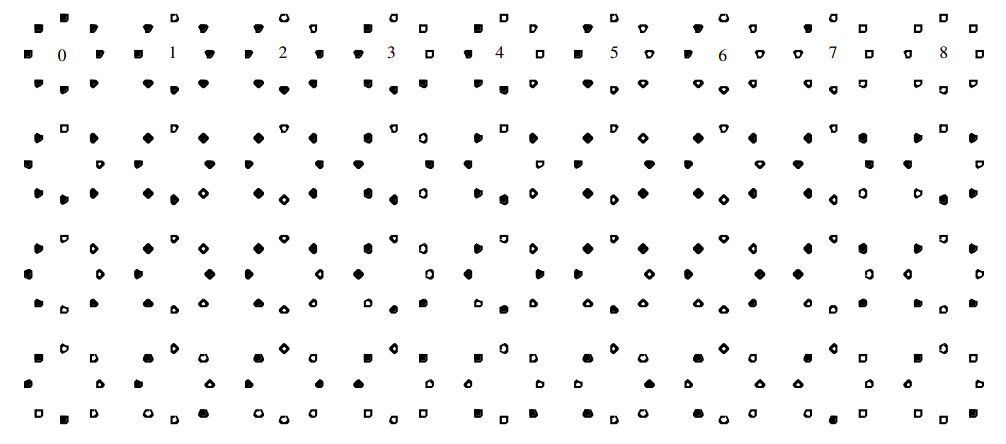
\includegraphics[scale=0.4]{images/theo1/uniform_exam}
		\caption{36 mẫu nhị phân khác nhau của $LPB_{8,R}^{\text{  ri}}$}
	\end{center}
\end{figure}

\begin{equation}
	LBP_{P,R}^{\text{  }riu2}=\begin{cases}
		\sum_{p=0}^{P-1}{s(g_p-g_c)}  & U(LBP_{P,R}\leq 2)\\
		P + 1 & U(LBP_{P,R}) > 2
	\end{cases}
\end{equation}
\textit{Trong đó:}
$$
	U(LBP_{P,R})=\left\lvert s(g_{P-1} - g_c)-s(g_0-g_c)\right\rvert + \sum_{p=1}^{P-1}{\left\lvert s(g_p - g_c)-s(g_{p-1}-g_c)\right\rvert}
$$

\textit{Chú thích:} 
\begin{itemize}
	\item Hàm \textit{U} thể hiện số lần chuyển từ bit 0 sang bit 1 và ngược lại của các điểm trên đường tròn.
	\item \textit{LBP\textsubscript{P,R}\textsuperscript{riu2}} là số lượng bit 1 trên đường tròn nếu mẫu đang xét Uniform. Ngược lại, bằng P + 1 nếu mẫu không Uniform.
\end{itemize}
\pagebreak

\textit{Ví dụ:}
\begin{itemize}
	\item Uniform Pattern 
	$$
		LBP_{P,R}^{\text{  }riu2} = 5
	$$
	\begin{figure}[H]
		\begin{center}
			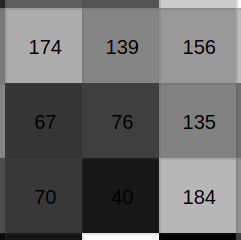
\includegraphics[scale=0.65]{images/theo1/LBP_exam4}
			\caption{Uniform Pattern}
		\end{center}
	\end{figure}
	\item Non-Uniform Pattern
	$$
		LBP_{P,R}^{\text{  }riu2} = 9
	$$
	\begin{figure}[H]
		\begin{center}
			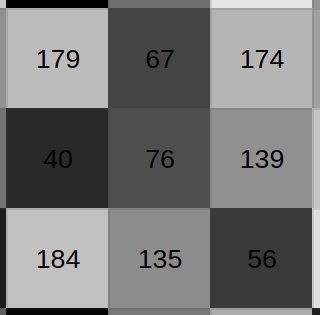
\includegraphics[scale=0.5]{images/theo1/LBP_exam1}
			\caption{Non-Uniform Pattern}
		\end{center}
	\end{figure}
\end{itemize}

\subsubsection{Adjacent Evaluation LBP (AELBP)}
\begin{equation}
	AELBP_{P,R}=\sum_{p=0}^{P-1}{s(a_p-g_c)\times 2^p}
\end{equation}
\textit{Trong đó:}
\begin{itemize}
	\item $a_p$ được tính bằng cách xem $g_p$ là tâm của một block(adjacent evaluation window) có kích thước W$\times$W (W cho trước). Sau đó, $a_p$ là giá trị trung bình của các điểm ảnh trong block đó (Không bao gồm $g_p$). Lưu lý W=1 thì AELBP có giá trị bằng với LBP.
\end{itemize}

\textit{Ví dụ:} Trong ví dụ dưới, ta chọn điểm $g_0$ tại góc trái trên, chiều quay ngược chiều lượng giác và W = 3. Song việc tính toán sẽ tương tự khi $g_0$ về góc lượng giác và chiều lượng giác như các phần trình bày trước.
$$
	AELBP_{P,R}=\sum_{p=0}^{P-1}{s(a_p-118)\times 2^p}=255
$$
\begin{figure}[H]
	\begin{center}
		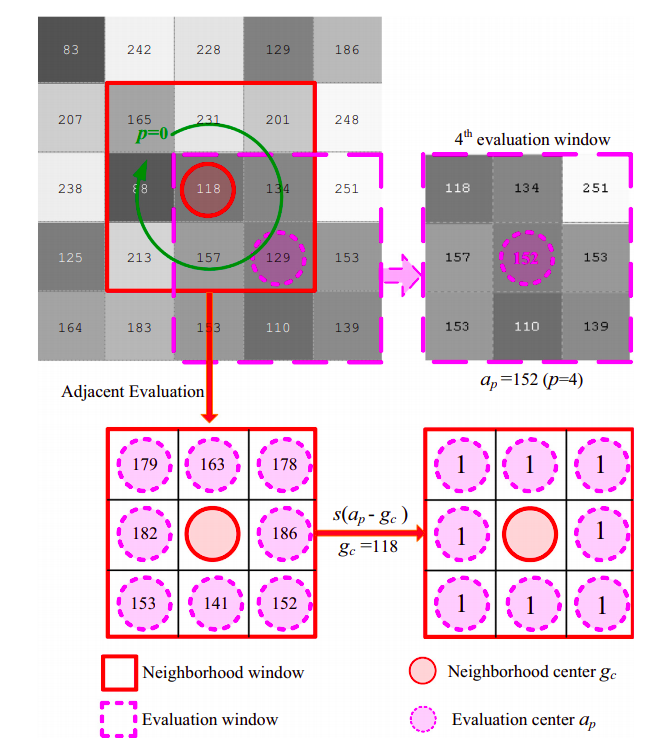
\includegraphics[scale=0.5]{images/theo1/AELBP}
		\caption{Ví dụ AELBP}
	\end{center}
\end{figure}

\underline{Ưu điểm}
\begin{itemize}
	\item AELBP có thể nhận dạng tốt các ảnh có nhiều noise, bằng cách sử dụng giá trị trung bình của lân cận với các điểm $g_p$. Trong khi LBP thông thường lại rất nhạy cảm với noise.
\end{itemize}
\underline{Nhược điểm}
\begin{itemize}
	\item Tính toán phức tạp hơn so với LBP thông thường.
\end{itemize}